%AUTOR: KAMIL ŁANGOWSKI 
%EMAIL: kamil.langowski@gmail.com
\documentclass[a4paper]{article}

\usepackage{polski}
\usepackage{amsfonts}
\usepackage{listings}
\usepackage{graphicx}
\usepackage{tikz}
\usepackage{geometry}


\lstdefinestyle{mystyle}{
    basicstyle=\ttfamily\footnotesize,
    breakatwhitespace=false,         
    breaklines=true,                 
    captionpos=b,                    
    keepspaces=true,                 
    numbers=left,                    
    numbersep=5pt,                  
    showspaces=false,                
    showstringspaces=false,
    showtabs=false,                  
    tabsize=2
}

\lstset{style=mystyle}

\title{Regresja liniowa}
\author{Kamil Łangowski \\ Wydział Fizyki Technicznej i Matematyki Stosowanej \\ Politechnika Gdańska}
\begin{document}
\maketitle
\newpage
\section{Teoria}

\subsection{Wstęp}
W tej części pracy omówimy jeden z najprostszych modeli w dziedzinie uczenia maszynowego, a zarazem jeden z najczęściej stosowanych. Jest to regresja liniowa (ang. \textit{linear regression}). Regresja liniowa jest modelem uczenia maszynowego nadzorowanego polegającym na wyznaczeniu funkcji, która z odpowiednią dokładnością wyznaczy zależność pomiędzy zmiennymi objaśniającymi a zmiennymi objaśnianymi. Aby móc mówić o regresji liniowej należy uprzednio założyć, że zależność pomiędzy zmiennymi, w dobrym przybliżeniu, jest liniowa. Zacznijmy od omówienia najbardziej fundamentalnego modelu, to znaczy prostej regresji liniowej.

\subsection{Prosta regresja liniowa}
W tym podejściu do modelu zakładamy, że mamy dwie zmienne $X= \{x_i\}_{i=1}^n$, gdzie $x_i \in \mathbb{R}$ i $Y = \{y_i\}_{i=1}^n$, $X$ jest zmienną objaśniającą , a $Y$ jest zmienną objaśnianą o charakterze ilościowym. Ponadto zakładamy, że zależność wiążąca funkcyjnie zmienną $Y$ ze zmienną $X$ jest w przybliżeniu liniowa. Oznacza to, że 
\begin{equation}\label{(3.1)}
    Y \approx \beta_0 + \beta_1X,
\end{equation}
gdzie $\beta_0$ i $\beta_1$ są nieznanymi parametrami równania reprezentującymi odpowiednio punkt przecięcia prostej z osią $OY$ (ang. \textit{intercept}) oraz współczynnik kierunkowy prostej (ang. \textit{slope}). Symbol "$\approx$" oddaje fakt, że zależność jest przybliżona, jednakże w dalszej części pracy, w celu przejrzystości używać będziemy symbolu równości. Określmy także kolejną prostą, której współczynniki oznaczone jako $\hat{\beta_0}$ i $\hat{\beta_1}$ będą estymowane na podstawie danych treningowych 
\begin{equation}\label{(2.2)}
    \hat{y} = \hat{\beta_0} + \hat{\beta_1}x,
\end{equation}
gdzie $\hat{y}$ jest wartością predykcyjną (przewidywaną) zmiennej $Y$  i $X = x$. Symbolem "$\;\hat{}\;$" oznaczamy zmienne, które estymują realne wartości.
\\\indent Zanim swobodnie będziemy mogli posługiwać się modelem, należy najpierw określić wartość parametrów $\beta_0$ i $\beta_1$ na podstawie posiadanych danych. Załóżmy, że mamy $n$ par obserwacji
\begin{equation}
(x_1, y_1), (x_2, y_2),\dots, (x_n, y_n),    
\end{equation}
gdzie $\forall_{i=1,\dots,n}(x_i, y_i)\in X\times Y$. Naszym celem jest znalezienie parametrów $\hat{\beta_0}$ i $\hat{\beta_1}$ takich, że model liniowy będzie w największym stopniu przybliżał dane z $n$-elementowej próbki. Oznacza to, że odległość punktów obserwacji $(x_i, y_i)$ dla $i = 1,2,\dots,n$ od prostej wyznaczonej przez równanie {(2)}
 ma być najmniejsza. Istnieją różne metody minimalizacji wspomnianej odległości m.in. metoda spadku gradientu (ang. \textit{gradient descent}), my jednak skupimy się na  metodzie, którą nosi nazwę metody najmniejszych kwadratów (ang. \textit{least squares}).

\subsection{Metoda najmniejszych kwadratów}
Niech $\forall_{i = 1,2,\dots,n}\;\hat{y}_i = \hat{\beta_0} + \hat{\beta_1}x_i\:$ będzie predykcją  $i$-tej etykiety na podstawie $i$-tej obserwacji z $X$. Zdefiniujmy 
\begin{equation}
k_i = y_i - \hat{y}_i,
\end{equation}
jako $i$-te rezyduum, czyli różnicę pomiędzy $i$-tą rzeczywistą wartością odpowiedzi, a $i$-tą wartością odpowiedzi przewidzianą przez nasz model.
\begin{figure}[ht]
    \centering
    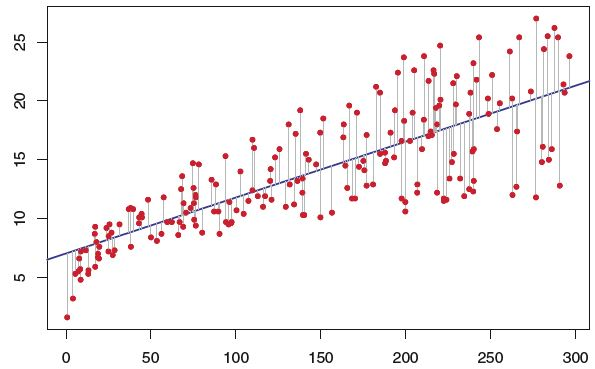
\includegraphics[]{MSE_ISLR.JPG}
    \caption{Na rysunku przedstawiono pewne obserwacje (czerwone punkty) oraz prostą regresji. W metodzie najmniejszych kwadratów chcemy aby suma kwadratów odległości punktów od prostej (szary odcinek)  była jak najmniejsza. Źródło: {ISLR}}.
\end{figure}\\
Wówczas możemy zdefiniować rezydualną sumę kwadratów (ang. \textit{residual sum of squares})
\begin{equation}
    \eta = k_1^2 + k_2^2 + \dots + k_n^2,
\end{equation}
lub
\begin{equation}
    \eta = \sum\limits_{i=1}^n{(y_i - \hat{\beta_0} - \hat{\beta_1}x_i)^2}.
\end{equation}
W metodzie najmniejszych kwadratów staramy się dobrać takie wartości współczynników $\hat{\beta_0}$, $\hat{\beta_1}$, aby rezydualna suma kwadratów $\eta$ była jak najmniejsza. Zdefiniujmy funkcję 
\begin{equation}
    J(\hat{\beta}_0, \hat{\beta}_1) = \sum\limits_{i=1}^n{(y_i - \hat{\beta_0} - \hat{\beta_1}x_i)^2}.
\end{equation}
W celu ustalenia minimum funkcji $J$ przyrównajmy jej pochodne cząstkowe do zera i wyznaczmy ekstrema
\begin{equation}
\left\{ \begin{array}{ll}
\frac{\partial{J}}{\partial{\hat{\beta_0}}} = (-2) \sum\limits_{i=1}^n{({y}_i - \hat{\beta_0} - \hat{\beta_1}x_i)} = 0 \\
\frac{\partial{J}}{\partial{\hat{\beta_1}}} = (-2) \sum\limits_{i=1}^n{({y}_i - \hat{\beta_0} - \hat{\beta_1}x_i)x_i} = 0
\end{array} \right.
\end{equation}
\begin{equation}
\left\{ \begin{array}{ll}
\sum\limits_{i=1}^n{({y}_i - \hat{\beta_0} - \hat{\beta_1}x_i)} = 0 \\
\sum\limits_{i=1}^n{({y}_i - \hat{\beta_0} - \hat{\beta_1}x_i)x_i} = 0
\end{array} \right.
\end{equation}
Przemnóżmy oba równania przez $\frac{1}{n}$
\begin{equation}
\left\{ \begin{array}{ll}
\frac{1}{n}\sum\limits_{i=1}^n{{y}_i} - \hat{\beta_0} - \hat{\beta_1}\frac{1}{n}\sum\limits_{i=1}^n{ x_i} = 0 \\

\frac{1}{n}\sum\limits_{i=1}^n{{y}_i x_i} - \hat{\beta_0}\frac{1}{n}\sum\limits_{i=1}^n{ x_i} - \hat{\beta_1}\frac{1}{n}\sum\limits_{i=1}^n{ x_i^2} = 0
\end{array} \right.
\end{equation}
zdefiniujmy $\bar{y} = \frac{1}{n}\sum\limits_{i=1}^n{{y}_i}$ i  $\bar{x} = \frac{1}{n}\sum\limits_{i=1}^n{x_i}$. Wówczas
\begin{equation}\label{eq:(3.10)}
\left\{ \begin{array}{ll}
 \hat{\beta_0} =\bar{y} - \hat{\beta_1}\bar{x}  \\

\frac{1}{n}\sum\limits_{i=1}^n{{y}_i x_i} - \hat{\beta_0}\bar{x} - \hat{\beta_1}\frac{1}{n}\sum\limits_{i=1}^n{ x_i^2} = 0,
\end{array} \right.
\end{equation}
podstawmy  $\hat{\beta_0} =\bar{y} - \hat{\beta_1}\bar{x}$ do drugiego równania, wtedy
\begin{equation}
    \frac{1}{n}\sum\limits_{i=1}^n{{y}_i x_i} - \bar{x}\bar{y} + \hat{\beta_1}\bar{x}^2-\hat{\beta_1}\frac{1}{n}\sum\limits_{i=1}^n{ x_i^2}=0,
\end{equation}
po przekształceniach
\begin{equation}
    \hat{\beta_1} = \frac{\sum\limits_{i=1}^n{(x_i y_i - \bar{x}\bar{y})}}{\sum\limits_{i=1}^n{(x_i - \bar{x}^2)}},
\end{equation}
co można sprowadzić do postaci 
\begin{equation}\label{eq:(3.13)}
    \hat{\beta}_1 = \frac{\sum\limits_{i=1}^n{(x_i - \bar{x})(y_i - \bar{y})}}{\sum\limits_{i=1}^n{(x_i - \bar{x})^2}}.
\end{equation}
Ostatecznie na podstawie {(11)} i  {(14)} mamy

\begin{equation}\label{(3.14)}
\left\{ \begin{array}{ll}
    \hat{\beta}_1 = \frac{\sum\limits_{i=1}^n{(x_i - \bar{x})(y_i - \bar{y})}}{\sum\limits_{i=1}^n{(x_i - \bar{x})^2}} \\
    \hat{\beta_0} = \bar{y} - \hat{\beta_1}\bar{x}.
\end{array} \right.
\end{equation}
Wyznaczone w powyższy sposób parametry są najlepszymi estymatorami $\beta_0$ i  $\beta_1$ {mnk}{mnk1}. 


\subsection{Dokładność modelu}
W rzeczywistości zależność, którą modelujemy nie jest jednoznacznie liniowa, możemy zatem zapisać równanie {(1)} jako
\begin{equation}\label{(3.15)}
    Y = \beta_0 + \beta_1 X + \varepsilon,
\end{equation}
gdzie $\varepsilon$ to niezależne zmienne losowe o rozkładzie $\mathcal{N}(0,\sigma^2)$ oddające losowe czynniki, takie jak np. niedokładność aparatury pomiarowej, zaburzające liniowość modelu. Równanie {(16)} jest najlepszym przybliżeniem liniowym rzeczywistej zależności pomiędzy zmienną $Y$, a zmienną $X$.
\\\indent W trakcie pracy z danymi, w większości przypadków, nie znamy równania regresji liniowej populacji. Z tego powodu posługujemy się równaniem {(2)} ze współczynnikami określonymi w {(15)}. Równanie to, na podstawie próbki z populacji w mniej lub bardziej odpowiedni sposób ukazuje nam kształt poszukiwanej zależności. Należy odnotować także fakt, że dla różnych próbek z jednej populacji kształt krzywej wyznaczonej przez {(2)} będzie się różnił, natomiast krzywa {(16)} pozostanie niezmienna. 
\\\indent W celu lepszego zrozumienia różnicy pomiędzy równaniami {(2)} i  {(16)} posłużmy się przykładem. Załóżmy, że chcemy poznać średnią populacji $\mu$ zmiennej $Y$. Powiedzmy także, że nie znamy wszystkich danych z $Y$, a jedynie próbkę $(y_1, y_2, \dots, y_l)$ o liczebności $l$. Możemy zatem skorzystać z tej próbki w celu estymacji wartości średniej $\mu$ dla całej populacji, oczywiście pod warunkiem, że próbka będzie odpowiednio liczna. Niech $\hat{\mu} = \sum_{i=1}^l{y_i}$ będzie średnią z próbki. Oczywistym jest, że średnia $\hat{\mu}$ i średnia ${\mu}$ będą się różniły, jednakże na ogół średnia odpowiednio liczebnej próbki statystycznej będzie dobrym estymatorem dla średniej populacji\footnote{Fakt ten znajduje uzasadnienie w prawach wielkich liczb.}. W ten sam sposób parametry $\hat{\beta_0}$ i $\hat{\beta_1}$ estymują (przybliżają) równanie {(16)}.


\subsection{Wielowymiarowa regresja liniowa}
Wielowymiarowa regresja liniowa (ang. \textit{multiple linear regression}) to naturalne rozwinięcie idei prostej regresji liniowej, w której predykcji dokonujemy na podstawie $d$ zmiennych objaśniających. We wielowymiarowej regresji liniowej mamy do czynienia z sytuacją, w której występuje zależność (w przybliżeniu liniowa) pomiędzy $d$ własnościami opisującymi przedmiot badania, a zmienną objaśnianą. Rozważaną zależność zapisujemy następująco 
\begin{equation}
    Y = \beta_0 + \sum\limits_{i=1}^d{\beta_iX^{(i)}} + \varepsilon,
\end{equation}
gdzie $X^{(i)}$ oznacza $i$-tą zmienną predykcyjną, a $\beta_i$ jest $i$-tym parametrem odpowiadającym $i$-tej zmiennej predykcyjnej. Podobnie jak w prostej regresji liniowej możemy posłużyć się metodą najmniejszych kwadratów w celu estymacji parametrów. Wtedy prosta regresji wyraża się wzorem
\begin{equation}
    \hat{y} = \hat{\beta_0} + \sum\limits_{i=1}^d{\hat{\beta_i}x^{(i)}},
\end{equation}
gdzie $x^{(i)} = X^{(i)}$. Z kolei rezydualna suma kwadratów przyjmuje kształt  
\begin{equation}
    \eta = \sum\limits_{i=1}^n{(y_i - \hat{y_i})^2}
\end{equation}
lub
\begin{equation}
    \eta = \sum\limits_{i=1}^n{(y_i - \hat{\beta_{0}} -\hat{\beta_{1}}x_{i}^{(1)} -\dots-\hat{\beta_{d}}x_{i}^{(d)})^2}.
\end{equation}
Określenie wartości parametrów odbywa się poprzez minimalizację funkcji 
\begin{equation}
    J(\hat{\beta_{0}},\hat{\beta_{1}}, \dots,\hat{\beta_{d}}) = \sum\limits_{i=1}^n{(y_i - \hat{\beta_{0}} -\hat{\beta_{1}}x_{i}^{(1)} -\dots-\hat{\beta_{d}}x_{i}^{(d)})^2}.
\end{equation}
Wzory na parametry $\hat{\beta_i}$ są jednak bardziej złożone niż dla prostej regresji liniowej i z tego względu nie będziemy ich przytaczać. Zagadnienie wielowymiarowej regresji liniowej częściej pojawia się w praktyce, gdyż zbiory danych na ogół zawierają więcej niż jedną zmienną predykcyjną. 

\section{Przykład}
\subsection{Opis zbioru}
Będziemy operować na zbiorze danych \textit{gapminder} wbudowanego do pakietu \textit{gapminder}. Zbiór zawiera dane na temat oczekiwanej dalszej długość trwania życia, PKB per capita oraz populacji poszczególnych krajów ze wszystkich kontynentów, badane co pięć lat od roku 1952 do roku 2007.

\subsection{Cel}
W przykładzie znajdziemy prostą regresji liniowej (jej współczynniki), która wyrażać będzie zależność przewidywanej długości życia w wybranym kraju (w tym przypadku Japonii) od roku, w którym wykonano badanie.

\subsection{Kod programu}
W pierwszym korku ładujemy pakiety, które będziemy używali w przykładzie:
\begin{lstlisting}[language=R, frame=single]
library(gapminder)
library(caret)
library(modelr)
library(tidyverse)
\end{lstlisting}
Pakiet \textit{gapminder} zawiera zbiór danych, na którym pracujemy. \textit{caret} -- to pakiet zawierający wiele przydatnych narzędzi do pracy z danymi, wizualizacji oraz tworzenia modeli uczenia maszynowego.  Pakiet \textit{tidyverse} zawieraja funkcję filtrującą. Przypisujemy zbiór do nazwy \textit{dane} i wyświetlamy  jego strukturę oraz podsumowanie informacji na temat każdego atrybutu:
\begin{lstlisting}[language=R,frame=single]
dane <- gapminder

str(dane)
summary(dane)
\end{lstlisting}
\begin{lstlisting}[language=R,frame=single]
tibble [1,704 x 6] (S3: tbl_df/tbl/data.frame)
 $ country  : Factor w/ 142 levels "Afghanistan",..: 1 1 1 1 1 1 1 1 1 1 ...
 $ continent: Factor w/ 5 levels "Africa","Americas",..: 3 3 3 3 3 3 3 3 3 3 ...
 $ year     : int [1:1704] 1952 1957 1962 1967 1972 1977 1982 1987 1992 1997 ...
 $ lifeExp  : num [1:1704] 28.8 30.3 32 34 36.1 ...
 $ pop      : int [1:1704] 8425333 9240934 10267083 11537966 13079460 14880372 12881816 13867957 16317921 22227415 ...
 $ gdpPercap: num [1:1704] 779 821 853 836 740 ...
 
         country        continent        year         lifeExp           pop           
 Afghanistan:  12   Africa  :624   Min.   :1952   Min.   :23.60   Min.   :6.001e+04  
 Albania    :  12   Americas:300   1st Qu.:1966   1st Qu.:48.20   1st Qu.:2.794e+06  
 Algeria    :  12   Asia    :396   Median :1980   Median :60.71   Median :7.024e+06  
 Angola     :  12   Europe  :360   Mean   :1980   Mean   :59.47   Mean   :2.960e+07  
 Argentina  :  12   Oceania : 24   3rd Qu.:1993   3rd Qu.:70.85   3rd Qu.:1.959e+07  
 Australia  :  12                  Max.   :2007   Max.   :82.60   Max.   :1.319e+09  
 (Other)    :1632                                                                    
   gdpPercap       
 Min.   :   241.2  
 1st Qu.:  1202.1  
 Median :  3531.8  
 Mean   :  7215.3  
 3rd Qu.:  9325.5  
 Max.   :113523.1 
\end{lstlisting}
Widzimy, że zbiór zawiera 1704 wiersze i 6 kolumn, są to kolejno:
\begin{itemize}
    \item \textit{country} -- nazwa kraju (zmienna kategoryczna),
    \item \textit{continent} -- nazwa kontynentu (zmienna kategoryczna),
    \item \textit{year} -- rok badania (zmienna całkowitoliczbowa),
    \item \textit{lifeExp} --   oczekiwana  dalsza  długość  trwania  życia (zmienna numeryczna), 
    \item \textit{pop} -- populacja (zmienna całkowitoliczbowa),
    \item \textit{gdpPercap} -- PKB per capita (zmienna numeryczna)
\end{itemize}
Naszą zmienną celu będzie \textit{lifeExp}, a zmienną objaśniającą \textit{year}. Wyświetlamy wykres zależności  \textit{lifeExp} od roku \textit{year} dla wszystkich krajów:
\begin{lstlisting}[language=R,frame=single]
ggplot(gapm, aes(year, lifeExp, group = country)) 
        + geom_line()
\end{lstlisting}
\begin{figure}[ht]
    \centering
    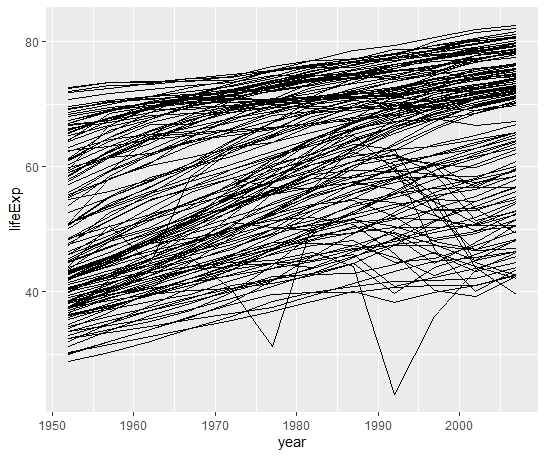
\includegraphics[width = 300  pt]{WSZYSTKIEKRAJE.jpeg}
    \caption{Wykres zależności pomiędzy rokiem badania, a przewidywaną długością życia.}
\end{figure}
Uzyskany wykres jest bardzo nieczytelny, jednak można wyciągnąć wniosek, że dla pewnych krajów zachodzi liniowość pomiędzy rozważanymi zmiennymi. Ograniczmy się w swoich rozważaniach do danych uzyskanych w Japonii. W tym celu tworzymy zmienną \textit{jap} przechowującą dane z Japonii oraz za pomocą środowiska \textit{ggplot} z pakietu \textit{caret} wyświetlamy dane na wykresie:
\begin{lstlisting}[language=R,frame=single]
jap <- filter (dane, country == 'Japan')
ggplot(jap, aes(year,lifeExp)) + geom_point(size = 3, colour = 'red')
\end{lstlisting}
\begin{figure}[ht]
    \centering
    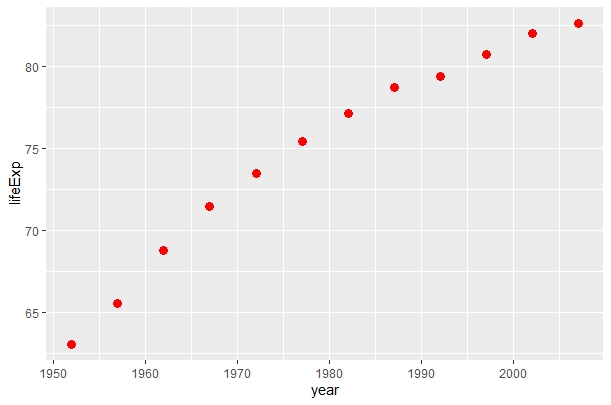
\includegraphics[width = 250 pt, height = 190 pt]{JAPONIA_PUNKTY.jpeg}
    \caption{Wykres badanej zależności dla Japonii.}
    \label{r(2.3)}
\end{figure}\newpage
W celu stworzenia modelu (wyznaczenia współczynników $\hat{\beta_0}, \hat{\beta_1}$) prostej regresji liniowej posłużymy się funkcją \textit{lm}, która bazuje na metodzie najmniejszych kwadratów. Tworzymy model i wyświetlamy jego parametry: 
\begin{lstlisting}[language=R, frame=single, ]
model <- lm(formula = lifeExp ~ year, data = jap)
coef(model)
\end{lstlisting}
\begin{lstlisting}[language=R, frame=single, ]
 (Intercept)         year 
-623.7469389    0.3529042 
\end{lstlisting}
Parametr \textit{(Intercept)} utożsamiamy z $\hat{\beta_0}$, a \textit{year} z $\hat{\beta_1}$, zatem nasza prosta wyraża się wzorem 
\begin{equation}
    y = -623.7469389 + 0.3529042x.
\end{equation}
Nakładamy wykres powyższej prostej na wykres z rys. \ref{r(2.3)}
\begin{lstlisting}[language=R, frame=single ]
ggplot(jap, aes(year, lifeExp)) +   geom_point(size = 3, colour = 'red') + 
geom_abline( aes(intercept = model$coefficients[1], slope = model$coefficients[2]), colour = 'blue', size = 1)
\end{lstlisting}
\begin{figure}[ht]
    \centering
    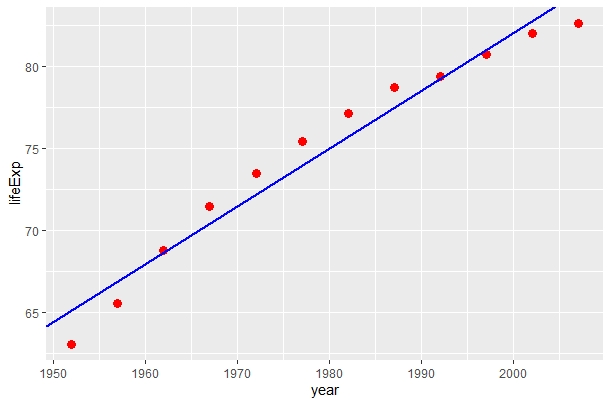
\includegraphics[width = 250 pt, height = 200 pt]{KRZYWA_REGRESJI.jpeg}
    \caption{Wykres modelu regresji liniowej opartego na metodzie najmniejszych kwadratów.}
    \label{r(2.4)}
\end{figure}
Krzywa z rysunku \ref{r(2.4)} obrazuje najlepsze przybliżenie liniowe zależności pomiędzy zmienną \textit{year}, a zmienną \textit{lifeExp}. W celu oceny modelu wyznaczmy błędy modelu rozumiane jako różnica pomiędzy wartością rzeczywistą \textit{lifeExp}, a wartością uzyskaną na drodze predykcji: 
\begin{lstlisting}[language=R, frame=single ]
residuals(model)
\end{lstlisting}
\begin{lstlisting}[language=R, frame=single ]
          1           2           3           4           5           6           7 
-2.09205128 -1.38657226  0.07890676  1.01438578  1.23986480  1.43534382  1.40082284 
          8           9          10          11          12 
 1.19630186  0.12178089 -0.31274009 -0.76726107 -1.92878205 
\end{lstlisting}
Liczby od 1 do 12 oznaczają różnicę dla kolejnych obserwacji począwszy od obserwacji z roku 1952. Widzimy, że największy błąd modelu to około 2 lata różnicy w szacowanej dalszej długości życia (pomiar pierwszy).


\end{document}